\section{共享风险链路组不相交路径对问题}
\subsection{问题描述}
\begin{frame}{目录}
    \setbeamertemplate{section in toc}[sections numbered]
    \tableofcontents[currentsection,hideothersubsections]
\end{frame}
\addtocounter{framenumber}{-1}  %目录页不计算页码

\begin{frame}
\frametitle{复杂多约束}
  \begin{itemize}
    \item 容量约束:链路上的占用带宽不得大于链路自身容量
    \item 端到端时延小于预定时延
    \item 端到端跳数不能超过预定跳数
    \item 路径必须有序地经过某些节点和链路
  \end{itemize}
\end{frame}

\begin{frame}
\frametitle{可生存性需求约束}
抗故障路由设计需要为业务流寻找工作路径和保护路径,多条路径满足分离要求
\begin{itemize}
  \item 链路分离:工作与保护路径经过的链路互不相同
  \item 节点分离:工作与保护路径经过的节点互不相同。节点分离必定链路分离
  \item 风险共享链路组(shared risk link group SRLG)分离:工作路径的风险共享链路组集合与保护路径的风险共享链路组集合没有交集
\end{itemize}
\end{frame}

\begin{frame}
\frametitle{多种优化目标}
\begin{itemize}
  \item Min-min disjoint paths problem
  \item Min-max disjoint paths problem
  \item Bounded disjoint paths problem
  \item Min-sum disjoint paths problem
\end{itemize}
\end{frame}

\begin{frame}
\frametitle{Min-Min SRLG不相交路径对问题}
给定一个图$G(V,E)$,每条链路$e_i\in \mathbb{E}$ 相关联一个权重$w_{e_i}$,一个源节点$s$和一个目的节点$d$,找到一对从$s$ 到$d$ 的SRLG 不相交路径对(表示为AP 和BP),而且要求这两条不相交路径中路径权重较小的那条路径权重最小化,形式化如下:

\begin{equation}
\begin{array}{*{20}{c}}
   {\mathop {minimize}\limits_{AP,BP} } & {\min \left( {{w_{AP}},{w_{BP}}} \right)}  \\
   {subject\ to} & {{r_{AP}} \cap {r_{BP}}{\rm{ = }}\phi }  \\
   {} & {\mathbb{AP} \cap \mathbb{BP}{\rm{ = }}\phi }  \\
\end{array}
\label{eq:problem definition}
\end{equation}

即${w_{AP}}$ 和 ${w_{BP}}$是AP和BP的路径权重,$\mathbb{AP}$ 和 $\mathbb{BP}$分别是路径AP和BP 上的链路集,${r_{AP}}$ 和 ${r_{BP}}$分别是影响路径AP和BP的SRLG 集。
\end{frame}

\begin{frame}
\begin{figure}[htbp]
  \centering
  % Requires \usepackage{graphicx}
  \includegraphics[width=4.5in]{figures/CompositeGraph}
  \caption{SRLG不相交路径对}
  \label{fig:CompositeGraph}
\end{figure}
\end{frame}

\begin{frame}
\frametitle{复杂度规模}
\begin{theorem}
\label{le:lemma1}
    Min-Min SRLG-不相交路径对问题是 NP-complete.
\end{theorem}
\begin{proof}
Min-Min链路不相交路径对问题是NP-complete 的,Min-Min链路不相交路径问题是Min-Min SRLG不相交路径问题的子问题。设Min-Min SRLG不相交路径问题的复杂性为C(A),则NP-complete$\leq$C(A)。

Min-Min SRLG-不相交路径对问题可归约到停机问题。并且给定任意两条路径,很容易在多项式时间内判别这两条路径是否为SRLG 不相交路径。C(A)$\leq$NP-complete。 因此,A=NP-complete。
\end{proof}
\end{frame}


\subsection{陷阱问题}
\begin{frame}
\frametitle{陷阱问题}
\begin{figure}[htbp]
\centering
% Requires \usepackage{graphicx}
\includegraphics[width=4.0in]{figures/KSPproblem}
  \caption{演示KSP算法效率低下实例}
  \label{fig:KSPproblem}
\end{figure}
\end{frame}


\subsection{原有算法}
\begin{frame}
\frametitle{原有算法}
  \begin{enumerate}
  \item ILP:通过整数线性规划方程使这两条路径总的权重最小化。
  \item IQCP:因为任意0−-1整数线性规划方程,其中所有变量为0或1,原问题的整数线性规划方程可以表示为一个二次约束方程。
  \item KSP:找到第K短路作为候选AP路径,一个接一个地测试候选的AP路径是否有相应的SRLG不相交路径BP。
  \item CoSE:当AP遇到陷阱问题时,CoSE尝试进行简单而详尽的搜索,以找到一个SRLG集合。任何AP路径通过这个SRLG集都无法找到SRLG不相交的BP路径。基于这个SRLG集合,它拆分原问题并设计算法来求SRLG不相交路径对。
\end{enumerate}
\end{frame}



\subsection{分而治之的快速SRLG不相交路径对算法}
\subsubsection{分而治之}
\begin{frame}
\frametitle{设计思想}
\textbf{SRLG冲突链路集}

对于给定的AP没有SRLG不相交路径BP时,此时一个陷阱问题发生,AP 中可能存在一个子链路集,这样任何主路径通过这个链路集里所有的这些“问题”链路都不能找到一条相对应SRLG不相交BP路径,我们称这个子链路集为\textbf{SRLG 冲突链路集}。
\end{frame}
\begin{frame}
\frametitle{研究内容}
\begin{itemize}
  \item 如何确定冲突集
  \item 如何设计SRLG不相交路由算法
\end{itemize}
\end{frame}


\subsubsection{SRLG冲突链路集合}
\begin{frame}
\frametitle{创新性的设置链路容量值}
基于割集基础找到SRLG 冲突链路集,我们构造了一个新图$G^*$ ,如下所示。
\begin{enumerate}
  \item $G^*$与$G$的节点和链路拓扑关系一样。
  \item 跟每条链路$e_i$相关的链路权重$w_{e_i}$是跟其相对应图$G$中边的权重一样的。
  \item 我们使用公式\ref{eq:capacity principle}的准则设置每条边$e_i \in \mathbb{E}$相关的容量$c_{e_i}$。
\end{enumerate}
\begin{equation}
c_{e_i} = \left\{ {\begin{array}{*{20}{c}}
   1 & {e_i{\rm{ }} \in {\rm{ \mathbb{AP}}}}  \\
   {\left| \mathbb{AP} \right|+1} & {e_i{\rm{ }} \in {\rm{ \mathbb{E}}}{{\rm{\mathbb{R}}}}}  \\
   {\left| {{\rm\mathbb{AP}}} \right| + \left( {\left| {{\rm\mathbb{AP}}} \right| + 1} \right)\times \left| {{\rm{\mathbb{E}}}{{\rm{\mathbb{R}}}}} \right| + 1} & {otherwise}  \\
\end{array}} \right.
\label{eq:capacity principle}
\end{equation}
$\mathbb{AP}$指在图$G$中较小权重路径$AP$上所有链路的集合,和$\mathbb{\mathbb{ER}}$指不属于路径$AP$上的边但是与路径$AP$上的边共享风险的链路集合。
\end{frame}

\begin{frame}
  如图\ref{fig:CompositeGraph}(c)所示,路径$AP$的边集合$\mathbb{AP}=\{e_1,e_2,e_3,e_4$
$,e_5,e_6,e_7,e_8\}$, $\mathbb{\mathbb{ER}}=\{e_9,e_{11},e_{17},e_{13},e_{19}\}$。$|\mathbb{AP}|=8$, $|\mathbb{\mathbb{ER}}|=5$, $|\mathbb{AP}|+1=9$ 和 ${\left| {{\rm{\mathbb{AP}}}} \right| + \left( {\left| {{\rm{\mathbb{AP}}}} \right| + 1} \right)\times \left| {{\rm{\mathbb{E}}}{{\rm{\mathbb{R}}}}} \right| + 1}=54$。我们产生一个新图$G^*$如图\ref{fig:FlowStarGraph}所示,在图$G^*$中边的容量是根据公式(\ref{eq:capacity principle})所设置。
\begin{figure}[tp]
  \centering
  % Requires \usepackage{graphicx}
  \includegraphics[width=4.5in]{figures/FlowStarGraph}
  \caption{图$G^*$实例}\label{fig:FlowStarGraph}
\end{figure}
\end{frame}

\begin{frame}
\frametitle{相关证明}
\begin{lemma}
\label{le:lemma1}
    在图$G^*$中任何从$s$到$d$的路径必须经过在$\mathbb{AP}$ 或者 $\mathbb{\mathbb{ER}}$中边集合的一条边。
    %note:draw a picture to describe the proof
\end{lemma}
\begin{lemma}
\label{le:lemma2}
    图$G^*$的任何一条最大流的流值最多为$|\mathbb{AP}|+(|\mathbb{AP}|+1)\times|\mathbb{\mathbb{ER}}|$。
\end{lemma}
\begin{lemma}
\label{le:lemma3}
    图$G^*$最小割$\Phi$的边割集$\mathbb{L}_{\Phi}$上所有链路都在$\mathbb{AP}$ 或者$\mathbb{\mathbb{ER}}$ 中。
\end{lemma}
\begin{theorem}
    如果在图$G$中一个单元流阻塞了全部边割集$\mathbb{L}_{\Phi}$的所有边,则在原图中不会存在任何流经过这个图的割$\Phi$。
\label{th:block flow}
\end{theorem}
\end{frame}

\begin{frame}
根据定理\ref{th:block flow},最小SRLG冲突链路集问题可以描述为:查找AP 链路集上的最小链路子集,这些链路可以阻塞边割集$\mathbb{L}_{\Phi}$。
  \begin{figure}[htbp]
  \centering
  % Requires \usepackage{graphicx}
  \includegraphics[width=4.0in]{figures/MinCutStarGraph}
  \caption{图$G^*$的最小割实例}\label{fig:MinCutStarGraph}
  \label{fig:MinCutStarGraph}
\end{figure}
\end{frame}

\begin{frame}
\frametitle{分而治之并行运行}
最初,让$\mathbb{I}=\emptyset$ ${\mathbb{O}}=\emptyset$,原来的Min-Min SRLG不相交路径对问题可以用$\mathcal{P}(\emptyset,\emptyset)$ 表示。给定SRLG冲突链路集$\mathbb{T}=\{{e_1},{e_2}, \cdots ,{e_{\left| \mathbb{T} \right|}}\}$,原问题$\mathcal{P}(\emptyset,\emptyset)$可按以下步骤划分。

\begin{enumerate}
  \item 首先,$\mathcal{P}(\emptyset,\emptyset)$能被划分成两个子问题$\mathcal{P}(\emptyset,\{e_1\})$ 和 $\mathcal{P}(\{e_1\},\emptyset)$。
  \item 类似,$\mathcal{P}(\emptyset,\{e_1\})$能被划分成两个子问题 $\mathcal{P}(\{e_1,e_2\},\emptyset)$ 和 $\mathcal{P}(\{e_1\},\{e_2\})$。
  \item 这个划分步骤持续直到步骤$|\mathbb{T}|$,问题$\mathcal{P}(\{e_1,e_2,\cdots ,{e_{\left| \mathbb{T} \right|-1}}\},\emptyset)$ 进一步的拆分成两个子问题$\mathcal{P}(\{e_1,e_2,\cdots ,{e_{\left| \mathbb{T} \right|-1}}, {e_{\left| \mathbb{T} \right|}}\},\emptyset)$ 和 $\mathcal{P}(\{e_1,e_2,\cdots ,{e_{\left| \mathbb{T} \right|-1}}\},{e_{\left| \mathbb{T} \right|}})$。注意到,子问题$\mathcal{P}(\{e_1,e_2,\cdots ,{e_{\left| \mathbb{T} \right|-1}}, {e_{\left| \mathbb{T} \right|}}\},\emptyset)$是无解的。
\end{enumerate}

\end{frame}
\begin{frame}
\frametitle{SRLG不相交路由算法}
\begin{figure}[htbp]
\large{
\begin{equation*}
{\mathcal P}(\emptyset ,\emptyset )\left\{ {\begin{array}{*{20}{l}}
{{\mathcal P}(\{ e_2\} ,\emptyset )\left\{ {\begin{array}{*{20}{l}}
{{\mathcal P}(\{ e_2,e_5\} ,\emptyset )\left\{ {\begin{array}{*{20}{l}}
{{\mathcal P}(\{ e_2,e_5,e_6\} ,\emptyset )}\\
{\boxed{{\mathcal P}(\{ e_2,e_5\} ,\{ e_6\} )}}
\end{array}} \right.}\\
{\boxed{{\mathcal P}(\{ e_2\} ,\{ e_5\} )}}
\end{array}} \right.}\\
{\boxed{{\mathcal P}(\emptyset ,\{ e_2\} )}}
\end{array}} \right.
\end{equation*}
}
\caption{SRLG冲突链路集$\{ e_2,e_5,e_6\}$,分而治之的解决方案}
\label{fig:DividedConquer}
\end{figure}
\end{frame}

\begin{frame}
\begin{algorithm}[H]
\caption{Min-Min SRLG不相交路径对算法}
\tiny{
\begin{algorithmic}[1]
\label{alg:min-min}
%\caption{Main process of Algorithm}
\REQUIRE
$G$: 网络图;$s$: 源节点;$d$: 目的节点:$\mathbb{I}$:必过链路集;
$\mathbb{O}$: 必不过链路集\\
\ENSURE AP: 主路径;BP: 备用路径
\STATE $AP=\emptyset$, $BP=\emptyset, \mathbb{I}=\emptyset, \mathbb{O}=\emptyset$
\STATE $AP\leftarrow$ FIND$\_$AP$(G,s,d,\mathbb{I},\mathbb{O})$\label{alg:findap}
\IF{$AP\neq\emptyset$}
    \RETURN $BP\leftarrow$ FIND\_SRLG\_Disjoint\_BP$(G,s,d,AP)$\label{alg:findsrlgdisjointbp}
    \IF{$BP\neq\emptyset$}
        \RETURN {路径对 $(AP,BP)$}\label{alg:returnpathpair}
    \ELSE
        \STATE 找到SRLG冲突链路集 $\mathbb{T}$\label{alg:findsrlgconflictinglinkset}
        \STATE $\mathbb{T}\leftarrow \mathbb{T}-(\mathbb{I}\cup\mathbb{O})$
        %\IF{$\mathbb{T}\neq \emptyset$}
        \STATE {分而治之的并行执行\\
        \tiny{
        $\!\!\!\!\!\!\!\!\!\!\!\!\!\!\!\!\!\!\!\left\{ \begin{array}{l}
 \left( {A{P_1},B{P_1}} \right)={{Min-Min}}\left( {G,s,d,\mathbb{I} ,\mathbb{O}\cup\{ {t_1}\} } \right), \\
 \left( {A{P_2},B{P_2}} \right)={{Min-Min}}\left( {G,s,d,\mathbb{I}\cup\{ {t_1}\} ,\mathbb{O}\cup\{ {t_2}\} } \right), \\
 \left( {A{P_3},B{P_3}} \right)={{Min-Min}}\left( {G,s,d,\mathbb{I}\cup\{ {t_1},{t_2}\} ,\mathbb{O}\cup\{ {t_3}\} } \right), \\
  \cdots  \\
 \left( {A{P_{\left| \mathbb{T} \right|}},B{P_{\left| \mathbb{T} \right|}}} \right) = {{Min-Min}}\left( {G,s,d,\mathbb{I}\cup \{ {t_1},{t_2}, \cdots ,{t_{\left| \mathbb{T} \right| - 1}}\} ,\mathbb{O}\cup\{ {t_{\left| \mathbb{T} \right|}}\} } \right) \\
 \end{array} \right.$
 }
        }\label{alg:dividedandconquer}
        \STATE{  {$\!\!\!\!\!\!\!\!\!\!\!F\leftarrow$ FIND\_FEASIBLE$(( {A{P_1},B{P_1}} )),\cdots,( {A{P_{|\mathbb{T} |}},B{P_{| \mathbb{T} |}}} )$}}\label{alg:findfeasible}
        %\ENDIF
         \IF{$F\neq{\emptyset,\emptyset}$}
         \RETURN{路径对 $(AP,BP)$ 满足条件 $AP = \mathop {\arg \min }\limits_{AP} \left\{ F \right\}$}
        \ENDIF
    \ENDIF
\ENDIF
\end{algorithmic}
}
\end{algorithm}
\end{frame}

\subsection{算法性能评估及比较}
\begin{frame}
\frametitle{性能评估}
\begin{tabular}{c|c}
  \toprule
  算法 & 时间复杂度 \\
  \midrule
  % after \\: \hline or \cline{col1-col2} \cline{col3-col4} ...
  SCLS & $|\mathbb{T}|\times(|\mathbb{E}|+|\mathbb{V}|)\times log(|\mathbb{V}|)$ \\
  \hline
  CoSE & $\prod\limits_{i = 1}^{_{|\mathbb{T}|}} {\left| {SRL{G_i}} \right|}\times (|\mathbb{E}|+|\mathbb{V}|)\times log(|\mathbb{V}|)$ \\
  \hline
  KSP & $K\times ((|\mathbb{E}|+|\mathbb{V}|)\times log(|\mathbb{V}|))$,最糟糕的K值是$2^{|\mathbb{E}|}$ \\
  \bottomrule
\end{tabular}
\end{frame}

%\begin{frame}
%\frametitle{实验仿真}
%%所有实现都是在linux服务器上运行的,这个服务器配置Intel(R) Xeon(R) CPU E5-2620  2.00GHz(24 核)和32.00GB内存。为了测量计算时间,我们在所有实现的算法中插入一个定时器。%实验数据代码放置在github网址
%\begin{table}[htbp]
%\caption{SRLG拓扑数据}
%  \centering
%\footnotesize{  \begin{tabular}{*{18}{c}}
%\toprule
%拓扑 & 1 & 2 & 3 & 4 & 5 & 6& 7   \\
%\midrule
%点   &     527&      521    &      521     &    2023             &     451     &     521     &     449       \\
%边   &    4158 &  4052     &    4152      &   4142          &       2780   &      4052   &      2778    \\
%%Graph density  & 1.5\% &    1.49\% &   1.52\%  &  0.1\%  &   0.10\% &   1.41\%  &  1.5\% &   1.38\%   \\
%No.SRLG & 132 &  86   &  89  &  207        & 210  &  128  &   88    \\
%SRLG边比率 & 9.66\% & 6.16\% &   6.18\% &   14.94\%    &   22.55\%  &  9.65\% &   9.53\%     \\
%\bottomrule
%\end{tabular}
%}
%\label{tab:AllSample}
%\end{table}
%\end{frame}

\begin{frame}
\frametitle{实验结果}
\begin{figure}[htbp]
\centering
\begin{minipage}[t]{0.45\linewidth}
\centering
\includegraphics[width=2.25in]{figures/weight}
\caption{路径权重}
\label{fig:normalization weitgh sum}
\end{minipage}
\hfill
\begin{minipage}[t]{0.45\linewidth}
\centering
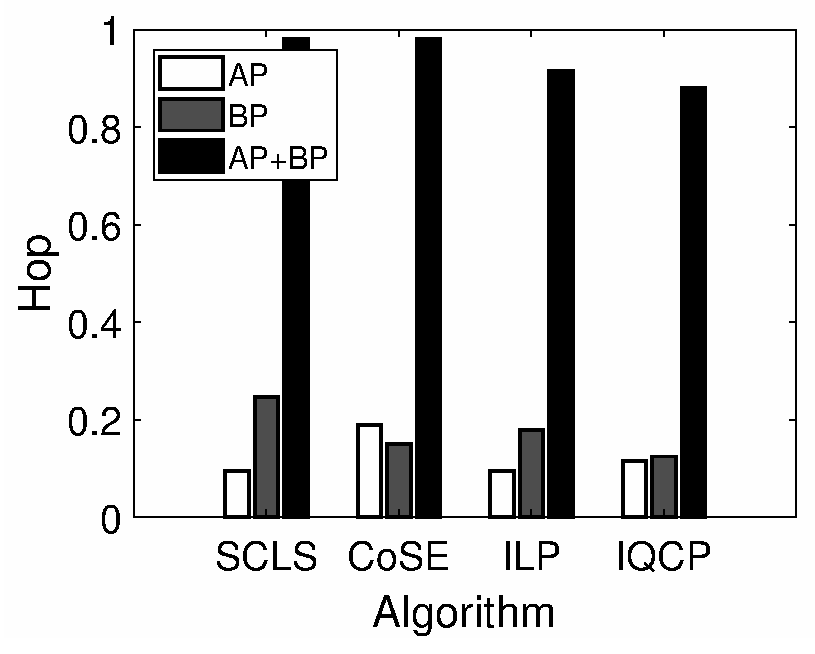
\includegraphics[width=2.25in]{figures/hop}
\caption{路径跳数}
\label{fig:normalization hop}
\end{minipage}
\end{figure}

\end{frame}





\begin{frame}
\begin{figure}[htbp]
\centering
\begin{minipage}[t]{0.3\linewidth}
\centering
\includegraphics[width=1.7in]{figures/runtime}
\caption{运行时间}
\label{fig:normalization runtime}
\end{minipage}
\hfill
\begin{minipage}[t]{0.3\linewidth}
\centering
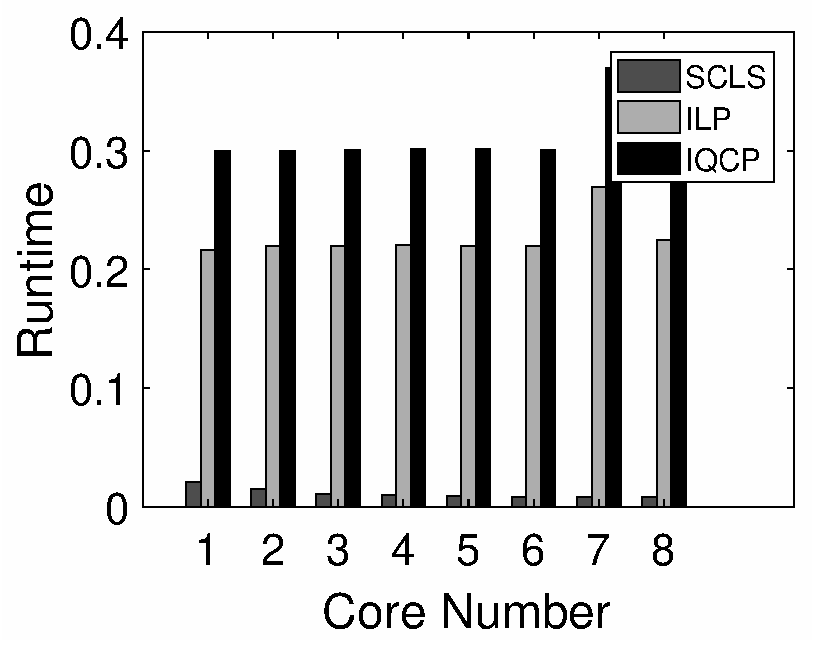
\includegraphics[width=1.7in]{figures/Runtime_noKSP_noCOSE}\\
  \caption{运行时间(无CoSE)}\label{fig:Runtime_noKSP_noCOSE}
\end{minipage}
\hfill
\begin{minipage}[t]{0.3\linewidth}
\centering
\includegraphics[width=1.7in]{figures/speedup}
\caption{核加速比}
\label{fig:Speedup}
\end{minipage}
\end{figure}
\end{frame}

\begin{frame}
\begin{figure}[htbp]
\centering
\begin{minipage}[t]{0.3\linewidth}
\centering
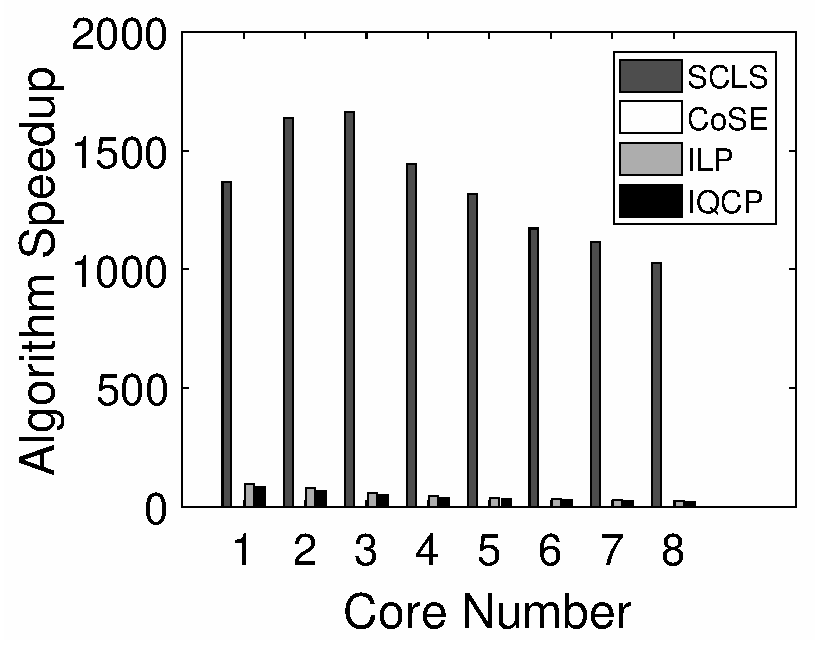
\includegraphics[width=1.7in]{figures/Multiple}
\caption{算法加速比}
\label{fig:Multiple}
\end{minipage}
\hfill
\begin{minipage}[t]{0.3\linewidth}
\centering
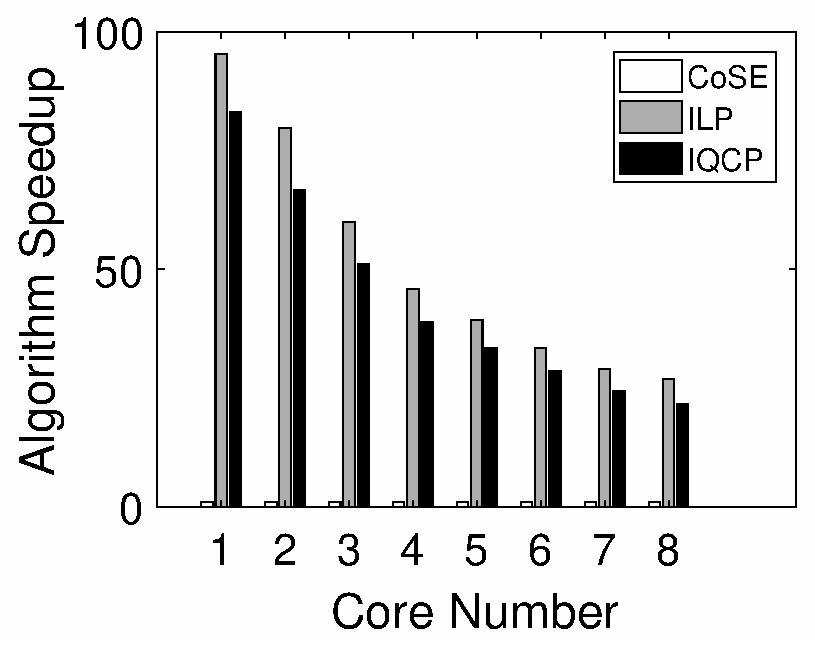
\includegraphics[width=1.7in]{figures/MultipleNoSCLS}
\caption{算法加速比(无SCLS)}
\label{fig:MultipleNoSCLS}
\end{minipage}
\hfill
\begin{minipage}[t]{0.3\linewidth}
\centering
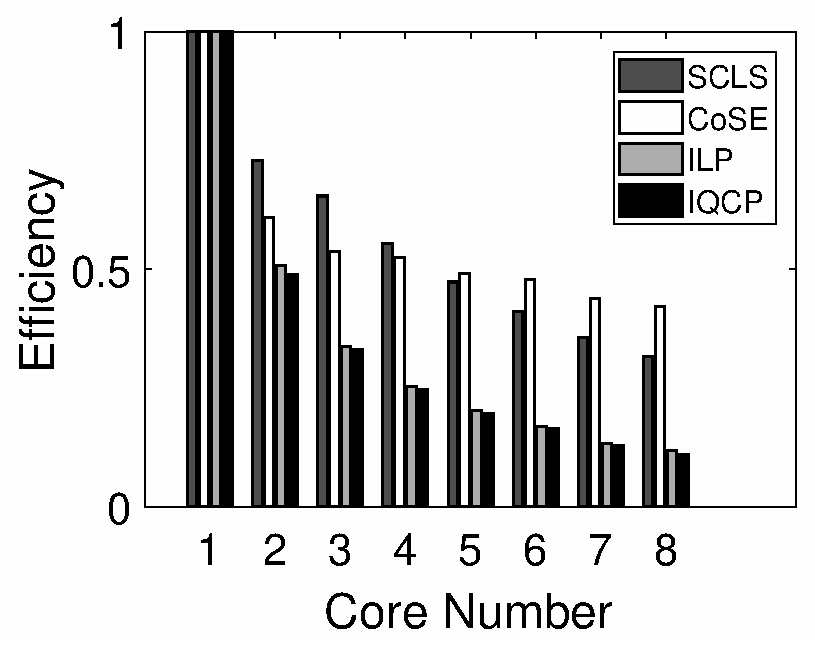
\includegraphics[width=1.7in]{figures/Efficiency}
 \caption{效率}
 \label{fig:Efficiency}
\end{minipage}
\end{figure}
\end{frame}
